\section{Specifications}
\subsection{Facebook Chatbot}
We are using facebook chatbot. So this picture can show you communicate among user, server, database. The information provided to the user is stored in the database so that the server provides information when needed.

\begin{figure}[htbp]
\centerline{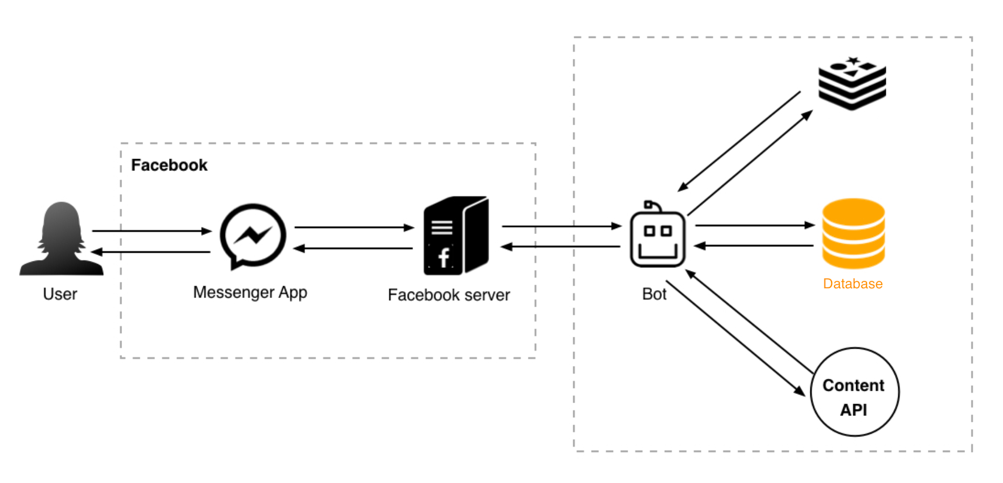
\includegraphics[width=\linewidth]{./pictures/facebook_overview}}
\caption{Overview of the system}
\label{fig}
\end{figure}
\FloatBarrier

If you are using Facebook Messenger, you don’t need a separate download. You can use the chatbot system by browsing the \emph{Before Order} page on Facebook, finding our page and clicking the Sending Message button.

\begin{figure}[htbp]
\centerline{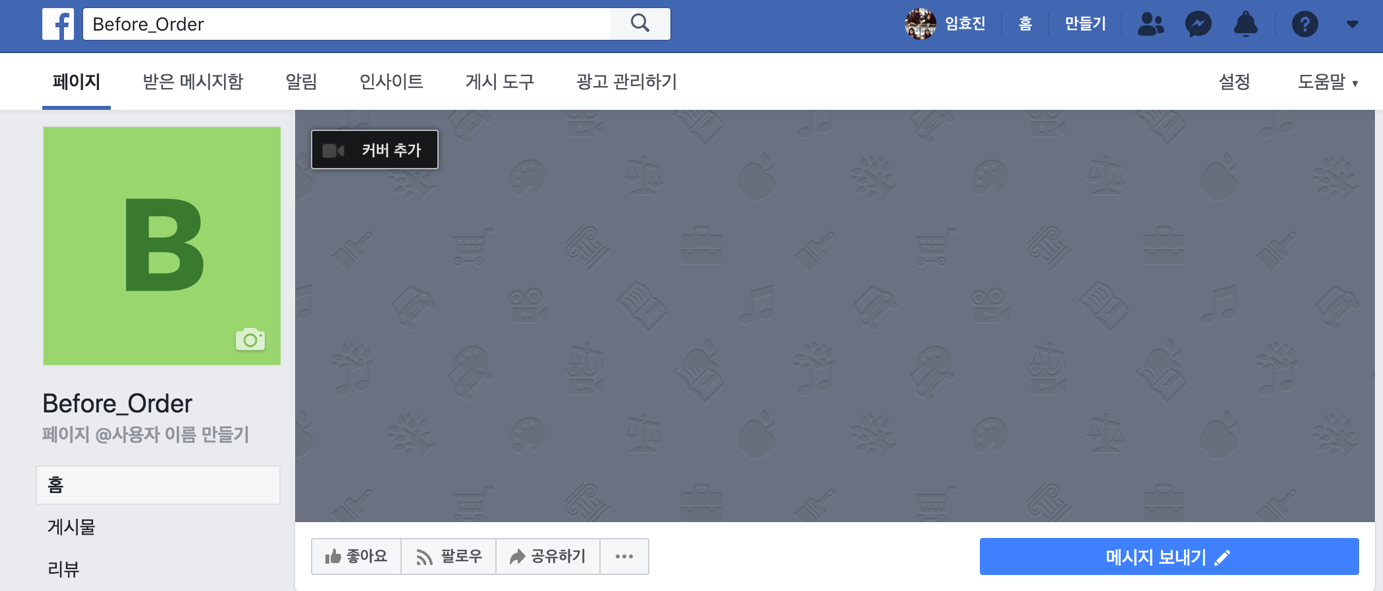
\includegraphics[width=\linewidth]{./pictures/facebook_profil}}
\caption{Chatbot profil on Facebook}
\label{fig:facebook_profil}
\end{figure}
\FloatBarrier

\subsubsection{Facebook messenger}

\begin{figure}[htbp]
\centerline{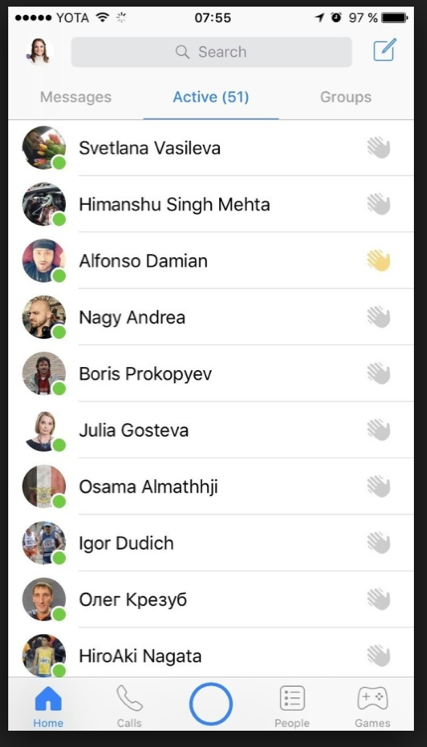
\includegraphics[width=\linewidth]{./pictures/facebook_friends}}
\caption{Homescreen of the Facebook Messenger}
\label{fig:facebook_friends}
\end{figure}
\FloatBarrier

If you select \emph{Before Order} from the messenger list, we ask you what information you need to provide information.

\begin{figure}[htbp]
\centerline{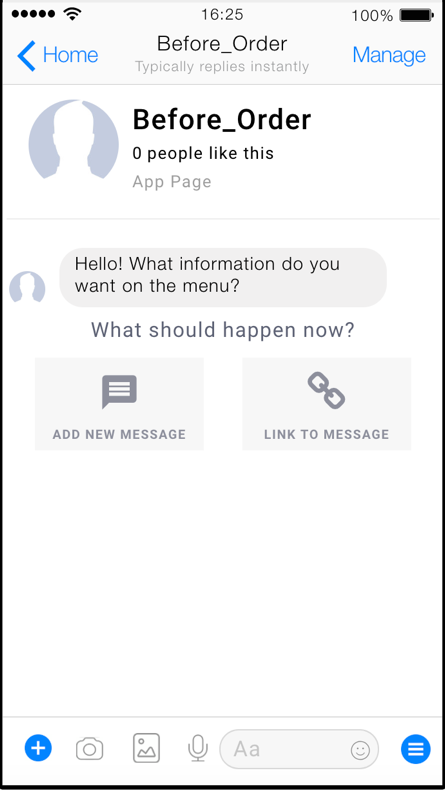
\includegraphics[width=\linewidth]{./pictures/facebook_message}}
\caption{Chatroom with the \emph{Before Order} chatbot}
\label{fig:facebook_message}
\end{figure}
\FloatBarrier

\subsubsection{Chatbot input}

The user sends a picture with the dishes written in letters. Most menus include no pictures of the dishes but only the names.

\begin{figure}[htbp]
\centerline{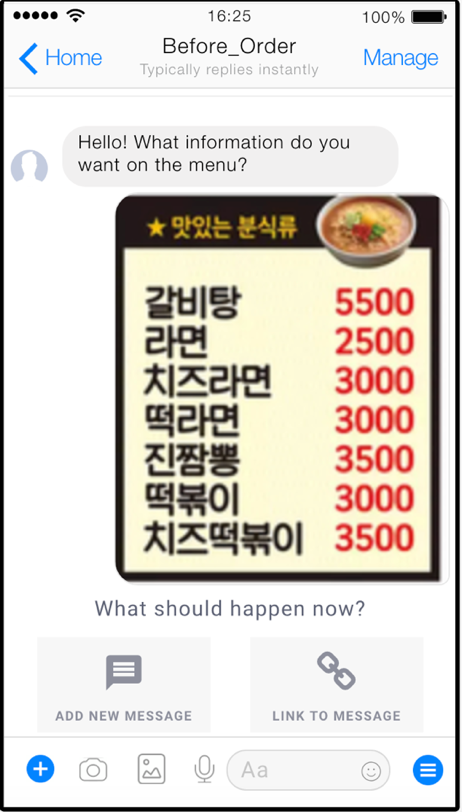
\includegraphics[width=\linewidth]{./pictures/facebook_menu}}
\caption{Message to the chatbot including a picture of a menu}
\label{fig:facebook_menu}
\end{figure}
\FloatBarrier

We provide a list of those letters using the text recognition API in the image and allow the user select from the list.

\begin{figure}[htbp]
\centerline{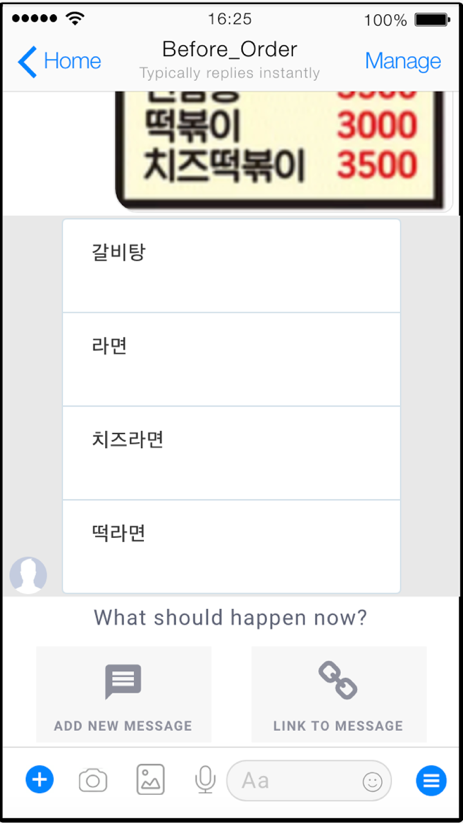
\includegraphics[width=\linewidth]{./pictures/facebook_response}}
\caption{Response of the chatbot with all the found dishes}
\label{fig:facebook_response}
\end{figure}
\FloatBarrier

The user selects the food for which information is to be provided in the list.

\begin{figure}[htbp]
\centerline{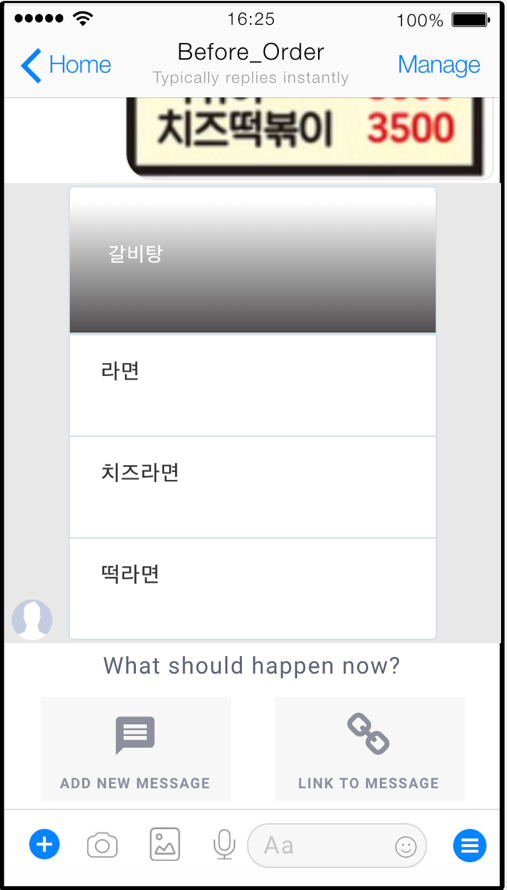
\includegraphics[width=\linewidth]{./pictures/facebook_response_selection}}
\caption{User selecting a dish from the list}
\label{fig:facebook_response_selection}
\end{figure}
\FloatBarrier

\subsubsection{Processing of the input}

\begin{itemize}
\item Get the information from database
\item Server that can run chat-bot
\item Vision api connection
\end{itemize}
\FloatBarrier

\subsubsection{Chatbot output}

\begin{figure}[htbp]
\centerline{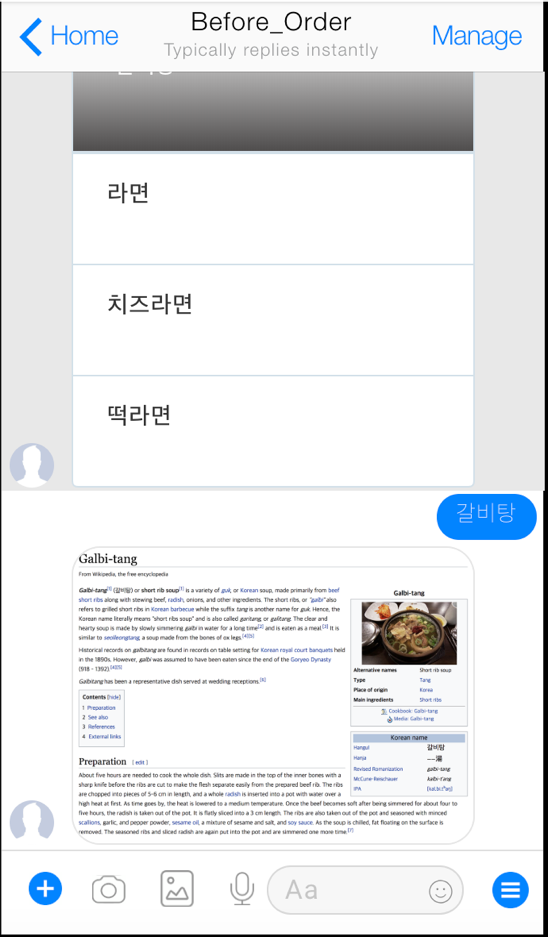
\includegraphics[width=\linewidth]{./pictures/facebook_dish_information}}
\caption{Detailed informations about the selected dish}
\label{fig:facebook_dish_information}
\end{figure}
\FloatBarrier

Although we can not represent it in this prototype, we plan to provide information from our internal database. Users can get photos, materials, and descriptions of food.

\subsubsection{Exit}
If you need information about other menus, please feel free to send us a message.